\section{Introduction}
\label{sec:introduction}

During their studies, students in the field of Banking and Finance learn a lot about asset management practices and theoretical business management aspects. To provide these students with an opportunity to apply their knowledge and understanding of the portfolio management process in practice, the Department of Banking of Finance offers the seminar ''Advanced Portfolio Management Game (S)'' every fall semester. During the seminar, students play a simulated game (''Portfolio management SIM'') in which they cooperate in teams to steer a bank's portfolio management and investment strategy as well as its business management of investment funds. Competition among the different student teams should make the learning process entertaining. \\

According to the Department of Banking and Finance, the game has the following key learning goals:
\begin{itemize}
  \item Students practice how money can be invested in financial markets in a systematic fashion.
  \item Students learn what factors make financial market forecasts possible and what limitations the applied models have for forecasting.
  \item Students learn which factors are relevant for the success (performance) of investments and can distinguish between factors that promise short-term and long-term success.
\end{itemize}

The game focuses on a structured investment process (as visualized in \Cref{fig:investment_process}). The process covers the steps from getting to know different customer types of the bank, selecting a suitable long-term Strategic Asset Allocation (SAA), adjusting it in the Tactical Asset Allocation (TAA) according to the status of the economy, and finally selecting appropriate titles matching SAA and TAA in the depot realization. In addition to these steps, the teams also decide on key business decisions like the salary to pay their employees and how much dividends to pay their shareholders.

\begin{figure}[h!]
  \centering
  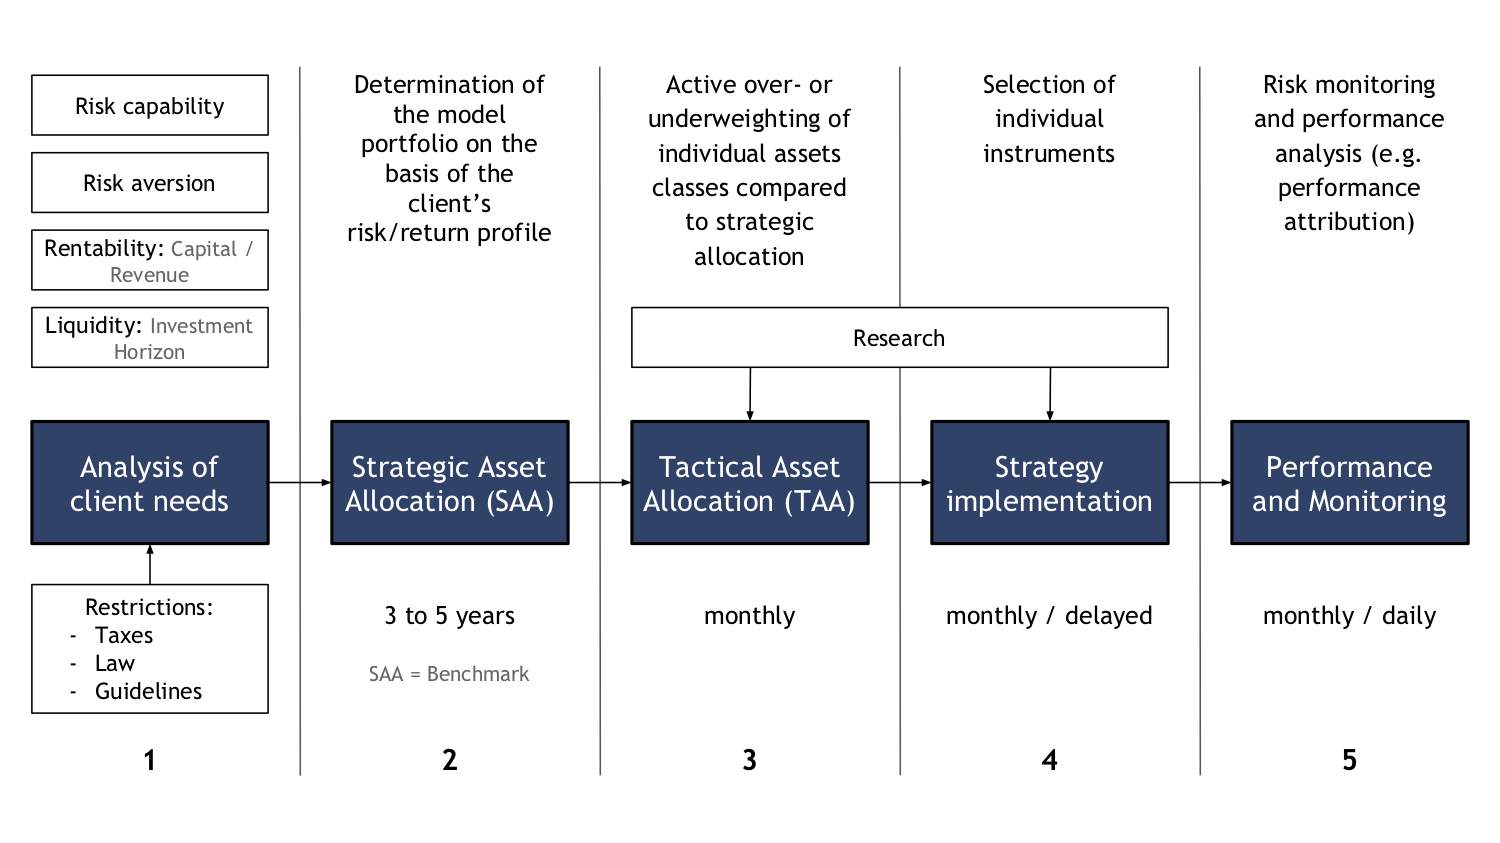
\includegraphics[scale=0.6]{img/private_banking_process.png}
  \caption{Overview of the structured investment process}
  \label{fig:investment_process}
\end{figure}

The currently used version of the ''Portfolio management SIM'' is both technically and didactically outdated. It was initiated in 2005 and initially developed by the Department of Banking and Finance at the University of Zurich in cooperation with the Swiss bank Julius Baer as well as the simulation development company game solution ag. Rapid technological development since that time enables new perspectives and possibilities in the field of game-based learning, which lead to the ideation of for this master project. \\

% TODO insert old game screenshots? not sure if helpful

The herein described master project (further referred to as the ''pfm-game'' project) aims to redesign and reprogram the existing ''Portfolio management SIM'' such that it is state-of-the-art from both a technical and didactical point of view. The project team assembled from students of the Departement of Informations and supervisors from both the Departement of Banking and Finance and Department of Informatics decided to cooperate on a modern version of the Portfolio Management Game. \\

The previous experience of the students in developing web applications, as well as their interest in analyzing financial processes and developing this game provides a solid foundation for the project. By re-developing the application, the Department of Banking and Finance wants to create a simulation of a typical portfolio management process that helps the students in their learning process by strengthening their practical decision making based on their theoretical knowledge. \\

The first section of this report (\Cref{sec:project_overview}) provides an overview of the ''pfm-game'' project and its scope and main goals, as well as a comparison with the existing ''Portfolio management SIM''. \Cref{sec:methodology} summarizes the approach to designing the new application by means of interviews, observation of games, and requirements engineering. The first technical section of this report (\Cref{sec:architecture}) then describes the main components of the technical application architecture and provides further references for interested readers. \\

A large part of this work that stays mainly in the background has been the implementation of a Python model that scores and evaluates the team decisions and handles large numbers of time-series. \Cref{sec:market_model} describes these efforts and how they integrate with the overall game such that future development could easily improve on the current version of this project. \Cref{sec:application_overview} then provides an overview over all key application interfaces and shortly summarizes their main intent and properties. As a final conclusion, \Cref{sec:conclusion} summarizes the progress made in this project as well as what is already planned and what could be imagined for future development.